\section{Feladatleírás}

A feladatunk egy algoritmus megtervezése, elkészítése, és tervezése, amely segítségével egy valós kamera felvételbe be lehet majd szúrni egy tetszőgeles virtuális geometriát, ami hihetően reagál a kamera mozgására, és a környezetére.
A feladat nehézsége miatt számos megszorítással, és feltétellel fogunk dolgozni, ezek a következőek:

\begin{itemize}
	\item A geometria a környezetéhez vett realtív pozíciója statikus, tahát a felvételen csak a kamera mozog
	\item A geometria nem reagál a környező fényhatásokra, nem lesz árnyékolva, és nem is vet árnyékot
	\item A felvétel előre fel lesz véve, az algoritmus nem feltétlenül lesz alkalmas valós idejű használatra
	\item A geometria kezdeti pozíciója előre, manuálisan meghatározott
\end{itemize}

\section{Megoldási lehetőségek\cite{yilmaz2006object}}

\subsection{Kálmán-szűrés}
A Kálmán-szűrő\cite{carvalho2021kalman} egy olyan rekurzió, amely a mozgó objektumok nyomon követésére egy x állapotvektor „legjobb” becslését adja, amely a cél paramétereit, például pozíciót tartalmazza. Ez egy olyan technika, amely megköveteli, hogy a tartalmazott statisztikai zaj, additív Gauss-zaj legyen, ennél a valós alkalmazásokban a zajkörnyezet bonyolultabb, így rossz becsléseket ad azokra az állapotváltozókra, amelyek nem követik a Gauss-eloszlást. Valós időben végrehajtható, előzetes információ nélkül, csak az aktuális bemeneti mérések és egy előre meghatározott bizonytalansági mátrix felhasználásával. A teljes szűrési folyamat egy predikciós és egy frissítési függvényből áll, amely a teljes rendszer ábrázolására is szolgál. Ezenkívül az állapotmodell lineáris.

\subsection{SORT algoritmus}
Kalmán-szűrővel kezeli az objektumok helyét egy videókockában és a magyar módszert használja adatkorreláció mérésére, csak akkor pontos, ha az objektum állapotbecslésének bizonytalansága alacsony, jó teljesítményt ér el akár magas képkockasebesség mellett is. A magyar algoritmus segítségével pontosan társítja a modellezett objektumokat, az objektumdetektor által gyűjtött friss adatokkal. Ezután a Kalmán-szűrő állapota az adott objektum alapján módosul, és az eljárás megismétlődik a következő képkockánál. A Deep-SORT metódus, amely integrálja az objektumok megjelenési információit, a SORT algoritmus továbbfejlesztett változata.

\subsection{Kiterjesztett Kálmán-szűrő\cite{strasdat2012local,zhang2018mobile}}
Pontkövetés az egymást követő képkockákban észlelt objektumokat pontok ábrázolják, és a pontok társítása az előző állapoton alapul, amely magában foglalja a helyzetét és mozgását. Lényegében az előző keretekből időbeli tartományban alkalmazott objektumszegmentálásnak tekinthetők. Az EKF az eredeti nemlineáris szűrődinamikának az előző állapotbecslések körüli linearizálásából származik. Míg a mozgáskövetés egy tárgy mozgásának követését jelenti a kamera szemszögéből, a kamerakövetés lényege a kamera pozíciójának követése egy fizikai térben. Mindkét megközelítés a mozgást és a szerkezetet a teljes háromdimenziós térben becsüli meg a képadatokból. 
Van néhány jelentős különbség az éles környezetben kevésbé sikeres EKF SLAM és az ORB SLAM2 között.\footnote{https://www.linkedin.com/pulse/what-im-learning-ekf-slam-orb-slam2-alex-thompson} A gyakorlatban a SLAM, a leképezés vagy a lokalizációs algoritmusok olyan folyamatot igényelnek, amely funkciókat biztosít, valamint módot a keretek között azok összeillesztésére. Az EKF SLAM, amikor mérési adatokat ad feltételezi, hogy a felismert tárgyhoz kapcsolódnak. Az ORB SLAM2 ezzel szemben elsősorban egy jellemzőazonosító és illesztési folyamat, amely minden kulcskockában felfedezi az ORB jellemzőket, és az ORB vektor alapján azonosítja az esetleges egyezéseket más kulcskockákban. Az EKF SLAM lényegében mindenkor frissíti az összes pontra vonatkozó jóslatot, még akkor is, ha messze van a kamera helyétől. Az ORB SLAM2 sokkal hatékonyabban a frissítéseket a lokálisra korlátozza, kivéve, ha konkrét mérések azt sugallják, hogy globális frissítésre van szükség. Körbejáráskor a leképezési algoritmusnak fel kell ismernie, hogy ezek a helyek megegyeznek, az EKF SLAM ezt úgy kezeli, hogy nem feltételezi, hogy az adatok ismertek, és folyamatosan frissíti az összes mutatót, az ORB SLAM2 egy egész rendszert valósít meg ennek a körülménynek a hatékony kezelésére.
\begin{figure*}
	\centering
	\captionsetup{justification=centering}
	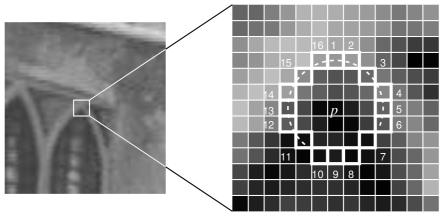
\includegraphics[width=1.7\columnwidth]{figs/fast_corner_detector.jpg}
	\vspace{-10pt}
	\caption{A FAST algoritmus egy lépése}
	\vspace{-10pt}
	\label{fig:FAST}
\end{figure*}


\section{ORB-SLAM}

\subsection{ORB-SLAM bevezető}

Az ORB-SLAM~\cite{7219438} egy monokulár SLAM rendszer, ami valós időben képes működni közel bármilyen környezetben. 
A SLAM (Simultaneous localization and mapping) rendszerek arra használhatók, hogy létrehozzunk és frissítsünk egy 3D-s térképet egy ismeretlen környezetről, miközben folyamatosan követjük a kamera pozícióját. 
Ebből is látható, hogy az általunk kitűzött célra tökéletes választás az ORB-SLAM.

Magának a rendszernek több verziója is létezik, technikai nehézségekből adódóan mi az ORB-SLAM 2-vel dolgozunk. 
A 2. és 3. verzió között követéspontossági eltérések vannak csak, az alapvető működésük egyforma. 
Amennyiben a fejlesztés során problémák adódnának a pontosságból, akkor az utolsó, javítási szakaszban át tudunk térni a 3. verzióra.

\subsection{ORB}

\subsubsection{ORB bevezető:}

Az ORB-SLAM az ORB~\cite{rublee2011orb} nevű keypoint detektáló, és megfeleltető algoritmusra épül, amelyet 2011-ben hoztak létre, hogy egy hatékony alternatívát biztosítson a SIFT~\cite{lowe2004distinctive}, illetve SURF~\cite{bay2006surf} megoldásokhoz.
A SIFT egy számításigényes, ugyanakkor magas pontosságú algoritmus, míg a SURF egy gyorsabb, viszont kevésbé megbízható opció.
Az ORB pontossága megközelíti a SIFT-ét, míg sebessége mindkét elődjét meghaladja.

Az ORB két algoritmus módosított verzióiból áll elő, ezek az oFAST, és az rBRIEF.

\subsubsection{FAST}


A FAST~\cite{rosten2006machine} detektor lényege, hogy egy 16 pontból álló kört vizsgál minden pixel körül.
Ezen 16 pixelből, ha N pixel világosabb, mint a kör közepén lévő pixel + egy küszöbérték, vagy pedig sötétebb, mint a kör közepén lévő pixel - egy küszöbérték, akkor a centrális pixel sarokpontnak tekinthető, ezt az \ref{fig:FAST}. ábra szemlélteti is.

Az algoritmus gyorsítható, hogyha a teljes környezet vizsgálata előtt néhány egyszerű teszt segítségével kiszűrjük az egyértelműen elvethető pontokat.
Első tesztként a 4 "fő-égtáj" (Észak, Kelet ...) menti pixelt vizsgálják, ami a mellékelt ábrán az 1, 5, 9 és 13 szám jelöl, ha ezek közül legalább 3 nem teljesíti a fenti feltételt, a pont elvethető.
Hasonló módon második tesztként a "mellék-égtájok" (Északkelet, Délkelete ...) menti pontok vizsgálandóak, azonos feltételek mellett.
Amennyiben a két előszűrési feltétel egyszerre teljesül, a kérdéses pont lehetséges sarokpont, és értelmes a teljes környezetét megvizsgálni.

Az algoritmus az alábbi problémákkal rendelkezik:

\begin{itemize}
	\item Nem általánosít jól N < 12 esetén.
	\item A teszthez használt pixelek és azok sorrendje implicit feltételezéseket tartalmaz a jellemzők megjelenésének eloszlásáról.
	\item Egyes megvalósítások esetén a 4 pont vizsgálata újra megtörténik a kör összes pontjának kiértékelésére során.
	\item Több egymás melletti sarokpont is észlelésre kerül.
	\item Számítőgép által generált, vagy nagyon tiszta élekkel rendelkező képeken nem működik jól
\end{itemize}

Az első 3 probléma hatási egy döntési fákra alapuló gépi tanulási eljárással csökkenthető.
Az eljárás során FAST algoritmust futtaták a tanításhoz használt képeken és megkeresik a sarokpont megállapítására legalkalmasabb pontokat.
A 4. problémára egy Non-maximal suppression eljárás van, ami minden lehetséges sarokponthoz rendel egy értéket, ami az abszolút különbség p és az őt körülvevő 16 pixel értéke között, majd az egymáshoz közel álló sarokpontok közül a kisebb értékkel rendelkezőket eltávolítja.
Az utolsó probléma egy Gauss filter alkalmazásával oldahtó meg, ami egyhény elmossa a túl éles sarokpontokat.

\subsubsection{BRIEF}

A BRIEF~\cite{calonder2010brief} egy jellemző leíró (feature descriptor), arra használható, hogy előre detektált kulcspontokhoz leíró adatokat rendelhessünk, például azok megkülönböztetése céljából.
A BRIEF az adott pontok/pixelek környezetéből készít bináris leírásokat, a következő képletek mentén:

$ f_{n_{d}}(p) := \sum_{1\leq i\leq n_{d}}^{}2^{i-1}\tau (p;x_{i},y_{i}) $

$ \tau (p;x,y)=\begin{Bmatrix}
	1 : p(x) < p(y) \\ 
	0 : p(x) \geq p(y)
\end{Bmatrix} $

Itt $ n_{d} $ a d. pont környezete, x és y egy pontpár p(x), illetve p(y) pedig a p környezet intenzitása az adott pontokon.
A két jellemző pont különböző véletlenszerű stratégiák mentén választható.

A BRIEF rendkívül gyors, és jól felismerhető leírásokat generál, gyengéje azonban, hogy nagyon érzékeny síkbeli forgatásokra.

\subsubsection{ORB részletek}

A fent említett alap algoritmusokra építve jött létre az ORB.

Első lépésként FAST pontokat detektál egy adott képen a FAST-9 (FAST 9-es rádiusszal) segítségével, majd ezt dolgozzák fel részletesebben az oFAST, azaz orientált FAST algoritmus segítségével.
A FAST nem készít "saroksági értéket", azaz nem adja meg, hogy egy adott pont mennyire biztosan valódi sarokpont.
A FAST e mellett gyakran jelez hibásan élek mentén, így szükséges a produkált pontokat a Harris sarokpont mértékük szerint sorba rendezni, majd az N "legsarokszerűbb" pontot kiválasztani közülük.
Az oFAST algoritmus kiemelt újdonsága, hogy a pontokhoz egy sarok orientációs értéket rendel az Intensity Centroid~\cite{rosin1999measuring} módszerrel.
Rosin egy patch momentumát a következő képpen határozza meg:

$ m_{pq} = \sum_{x,y}^{}x^{q}y^{q}I(x,y) $

Ezen momentumok segítségével határozzák meg a centroid pozícióját:

$ C = (\frac{m_{10}}{m_{00}},\frac{m_{01}}{m_{00}}) $

A centroid pozíciójának ismeretében meghatározható a vektor, illetve az arkusz tangens kvadráns biztos megfelelőjével meghatározható a patch iránya:

$ \Theta = atan2(m_{01},m_{10}) $

Az így meghatározott oFAST metódus rendkívül jól teljesít mesterségesen forgatott zajos adatokon is.

Az ORB algoritmus másik sarokköve a szintén fent említett BRIEF algoritmus rBRIEF nevű módosított változata.
Az eredeti BRIEF algoritmus teljesítménye sokat romlik, ha az adott képen síkbeli forgatást hajtunk végre, ezt két lépésben küszöbölték ki.
Először is az úgynevezett steered BRIEF algoritmust hozták létre, ami az oFAST során kiszámított sarok orientációkat felhasználva javítja a módszer forgatás invarianciáját.
Az így létrehozott featureknek azonban jelentősen csökken a varianciája, így nehezebb őket megkülönböztetni egymástól, hiszen közeli pontok featurejei hasonlóan fognak reagálni a különböző transzformációkra, így közel is maradnak egymáshoz.
A végső rBRIEF algoritmus egy mohó keresés során kiválasztja a legnagyobb varianciájú, nem összefüggő teszteket.

\subsection{ORB-SLAM részletek}

Az ORB-SLAM központi algoritmusa az úgynevezett Bundle Adjustment (BA). 
Ennek a lényege, hogy egyidőben történik a tér 3D geometriájának, a relatív mozgás paramétereinek és a kamera optikai tulajdonságainak finomítása.
Több módszer is használta a BA-t korábban, de az ORB-SLAM ezen felül több dolgot is csinál, többek között: 
\begin{itemize}
	\item Ugyanazokat a jellemzőket használja az összes feladathoz
	\item Covisibility gráf segítségével nagy környezetekben is képes valósidejű működésre
	\item Esszenciális gráf segítségével valós időben képes lezárni a köröket
\end{itemize}

\subsubsection{Az ORB-SLAM definíciói}

\textit{Térkép pont.} Minden $p_i$ térkép pont tartalmazza: az $X_{w, i}$ pozícióját a 3D-s térben, a megfigyelés $n_i$ irányát, a reprezentáns $D_i$ ORB leírót és a $d_{max}$ és $d_{min}$ távolságokat, amikből a pont megfigyelhető.

\textit{Keyframe.} Minden $K_i$ keyframe tartalmazza: a $T_iw$ kamera pózt, ami egy merev test transzformáció, ami a pontot a világ koordináta rendszerből a kamera koordináta rendszerébe transzformálja, a kamera paramétereit és minden ORB jellemzőt, amit a képkockából ki lehet nyerni. 

\textit{Covisibility gráf.} A Covisibility gráf egy súlyozott, irányítatlan gráf ami a keyframe-ek közötti láthatóságot reprezentálja. 
Minden csúcs egy keyframe, és két csúcs között akkor létezik él, ha mindkét keyframe tartalmaznak közös térkép pontokat (legalább 15-öt). 
Az él súlya pedig a közös képpontok száma ($\theta$).

\textit{Esszenciális gráf.} Az esszenciális gráf a covisibility gráfból készül: a csúcsok megegyeznek, viszont sokkal kevesebb éle van. 
Az esszenciális gráf a covisibility gráf feszítőfájából, a kört záró élekből és a covisibility gráf azon éleiből áll, ahol $\theta_{min} = 100$.

\subsubsection{Működés összefoglalva}
Az ORB-SLAM egyszerre három szálon fut: az egyiken történik a követés, a másikon a lokális mapping, a harmadikon pedig a kör bezárása.
A követés feladata, hogy a kamerát lokalizálja minden egyes képkockán, és eldöntse, hogy mikor szükséges új keyframe beszúrása.
A lokális mapping feldolgozza az új keyframe-eket, és lokális BA segítségével optimális módon rekonstruálja a környezetet.
A kör bezáró szál pedig minden új keyframe beszúrásakor kört keres az esszenciális gráfban, és amennyiben talál, akkor összeolvasztja a duplikált pontokat.

\subsubsection{Követés}

\textit{Automatikus térkép inicializálás.} A célja, hogy két képkockából meg tudja állapítani a kiindulási térkép pontokat.
Az ORB-SLAM ezt két módon teszi meg: homográfiával síkbeli esetet feltételezve, illetve fundamentális mátrixszal.
Ezt a két módszert párhuzamosan alkalmazza, és heurisztikával állapítja meg, hogy a két modell közül melyiket kell alkalmazni.
Az ORB-SLAM csak akkor fejezi be az inicializációt, amikor biztos benne, hogy helyes az eredmény - érzékelni tudja azokat az eseteket, amik helytelen kiindulási térképet eredményeznének.
Ez a következőképpen működik:
\begin{enumerate}
	\item Kinyeri az ORB jellemzőket az aktuális $F_c$ képkockából és $x_c \leftrightarrow x_r$ egyezéseket keres az $F_r$ referencia képkockával.
	\item Párhuzamosan kiszámolja a $H_{cr}$ homográfiát és az $F_{cr}$ fundamentális mátrixot a DLT és a 8 pontos algoritmusokkal.
	\item Kiszámol egy $S_M$ értéket minden $M$ modellhez (ahol $M = H$, ha homográfiáról van szó, egyébként $M = F$), több iteráción keresztül, és azt a homográfiát és fundamentális mátrixot tartja meg, aminek a legnagyobb az értéke. Ha ilyen nincs, akkor elölről kezdi az 1. lépéssel.
	\item Ha a környezet síkbeli, akkor a homográfiát érdemes választani, egyébként a fundamentális mátrixot. Ezt úgy dönti el, hogy kiszámol egy $R_H = \frac{S_H}{S_H + R_F}$ heurisztikát, és a homográfiát választja, ha $R_H > 0.45$.
	\item Elvégez egy teljes BA-t.
\end{enumerate}

\textit{Követés.} Maga a követés is több lépésből áll:
\begin{enumerate}
	\item \textit{ORB kinyerés.}  FAST sarkokat keresnek 8 skála szinten - kis felbontás esetén 1000, nagy felbontás esetén 2000 sarkot. Ehhez felosztják az egész képet egy négyzetrácsra, és minden cellából megpróbálnak 5 sarkot kinyerni, módosítva a felbontáson, ha nem sikerül. Ezekből aztán ORB leíró készül.
	\item \textit{Helyzet közelítés előző képkockából.} Ha a követés sikeres volt az előző képkockán, akkor konstans sebességű mozgási modellel előrejelzik a kamera helyzetét a következő képkockán, felhasználva ehhez az előző térkép pontokat. Ha sikertelen, akkor bővítik a keresési teret.
	\item \textit{Helyzet közelítés globális relokalizációval.} Ha a követés megszűnt, akkor az egész képkockát áttranszformálják egy Bag of Words-é és megpróbálják lekérdezni a lehetséges keyframe-eket egy felismerési adatbázisból, és ez alapján optimalizálják a pozíciót.
	\item \textit{Lokális térkép követése.} A lokális térkép tartalmazza azon $K_1$ keyframe-eket, amiknek van közös térkép pontjuk az aktuális képkockával, azon $K_2$ keyframe-eket, amik a $K_1$-beli elemek szomszédai a covisibility gráfon, illetve egy $K_{ref} \in K_1$ referencia keyframe-et, aminek a legtöbb közös pontja van az aktuális képkockával. Ezek alapján optimalizálják a kamera pozíciót.
	\item \textit{Új keyframe döntés.} Ha legalább 20 képkocka telt el a legutolsó globális relokalizáció óta, a lokális mapping jelenleg nem fut, az aktuális képkocka legalább 50 pontot követ, és ezek legfeljebb 90\%-a egyezik meg $K_{ref}$ pontjaival, akkor az aktuális képkocka bekerül a keyframe-ek közé.
\end{enumerate}

\subsubsection{Lokális mapping}

A lokális mapping során minden $K_i$ keyframe a következő lépéseken megy keresztül:

\begin{enumerate}
	\item \textit{Keyframe beillesztés.} $K_i$ új csúcsként bekerül a covisibility gráfba. Ezután frissítésre kerülnek a gráf élei és a feszítőfája, majd kiszámolják $K_i$ Bag of Words reprezentációját.
	\item \textit{Friss térkép pontok selejtezése.} Minden térkép pont 3 képkockával a létrejövése után egy teszten megy át: a követésnek meg kell találnia azon képkockák legalább 25\%-ában, amiből azt jósolta, hogy látható; illetve ha már legalább egy keyframe eltelt a létrejövése óta, akkor legalább 3 keyframe-ben megfigyelhetőnek kell lennie. Ha ezek teljesülnek, akkor a térkép pont csak akkor törlődhet, ha kevesebb, mint 3 keyframe-ből látható.
	\item \textit{Új térkép pontok gyártása.} Az epipoláris megkötés figyelembe vételével a covisibility gráf összekötött csúcsainak ORB leíróiból háromszögeléssel jönnek létre az új térkép pontok.
	\item \textit{Lokális BA.} A lokális BA optimalizálja az összes feldolgozott keyframe-et.
	\item \textit{Lokális keyframe-ek selejtezése.} A BA optimális működéséhez és a sokáig tartó futáshoz szükség van a redundáns keyframe-ek törlésére. Minden olyan keyframe törlésre kerül, amik térkép pontjainak legalább 90\%-át legalább 3 másik keyframe-ből is lehet látni.
\end{enumerate}

\subsubsection{Kör bezárása}

A kör bezárását végző szál veszi az utolsó feldolgozott keyframe-et ($K_i$), és lehetséges kört keres, és ha talál, akkor bezárja.
Ehhez a következő lépéseket hajtja végre:

\begin{enumerate}
	\item \textit{Lehetséges kör detektálása.} Ehhez veszik $K_i$ Bag of Words vektorát, illetve az összes szomszédját a covisibility gráfon, ahol $\theta_{min} = 30$. Ezután kiszámolják a keyframe-ek hasonlóságát, majd veszik annak $s_{min}$ minimumát. Minden olyan keyframe-et eldobnak, aminek az értéke $s_{min}$-nél kisebb, illetve közvetlenül össze van kötve $K_i$-vel. Ezután választanak egy lehetséges kört.
	\item \textit{Hasonlósági transzformáció kiszámítása.} Kiszámítanak egy hasonlósági transzformációt $K_i$ és egy lehetséges kör keyframe $K_l$ között. Ezzel ki tudják számolni a hibát, ami a kör létrehozásakor keletkezhetett.
	\item \textit{Kör összeolvasztása.} Itt összeolvasztják a duplikált térkép pontokat, és új éleket illesztenek be a covisibility gráfba, amivel be tudják zárni a kört. A korábban kiszámolt hasonlósági transzformáció segítségével korrigálják a hibákat, majd minden keyframe frissíti az éleit a covisibility gráfban.
	\item \textit{Esszenciális gráf optimalizáció.} A kör effektív lezárása érdekében szintén hasonlósági transzformációval optimalizálják az esszenciális gráfot. Ezután minden térkép pontra végrehajtják a transzformációkat.
\end{enumerate}

\section{Mapping}

Az ORB-SLAM miután végzett egy videó elemzésével létrehoz egy keyframeTrajectory.txt-t, amiben elmenti, hogy a kamera adott pillanatokban milyen pozícióba mozdult el a videó elején felvett pozíciójához képest.
Ez alapján a kimenet alapján már készítettek egy Match Move algoritmust, ami képes egy 3 dimenziós geometriát egy videóban elhelyezni.\footnote{https://github.com/ChiWeiHsiao/Match-Moving}
Mivel a kimenetben a kamera térbeli elhelyezkedése, és forgása is le van írva, így egyszerűen adódik, hogy a behelyezendő geometriát alávetjük a kamerán végrehajtott transzformációk inverzének, annak érdekében, hogy megkapjuk az új pozícióját.
Az általunk talált megoldásban a behelyezett geometria hamar elcsúszik az eredeti pozíciójáról, ennek oka, hogy a különböző keyframe-k közti mozgást nehéz pontosan megbecsülni.
Ezen felül azokat a frameket, amelyekre nem kaptak kész eredményt egyszerűen kihagyták.

Több javítási javaslatunk is van, először is az ORB-SLAM képes visszatérni az összes framere számított kamera pozícióval.
Ha ez mégsem lenne opció, akkor a keyframek közötti képek megtartásával, és egy maximum lehetséges eltolás bevezetésével korlátozzuk majd, a geometria csúszását.